% !TeX root = ../Skript_HTML.tex
\cohead{\Large\textbf{Listen}}
\section{Listen}
Damit man etwas mehr über den Webseitenersteller erfährt, soll die Webseite um zwei Listen nach folgendem Muster erweitert werden:
wissen, um wessen Website es sich dabei handelt. Daher soll eine Überschrift eingefügt werden.
\begin{minipage}[t]{\textwidth}
    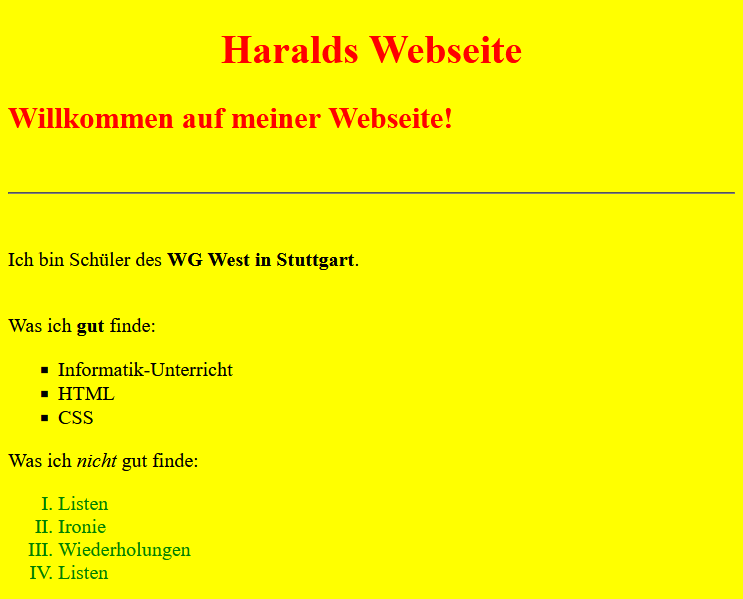
\includegraphics[width=\linewidth]{\pics/Listen.png}
\end{minipage}

\begin{Exercise}[title=, label=Listen]
    \begin{enumerate}
        \item Erweitere deine \textit{schueler.html} mit dem Windows-Editor entsprechend des obigen Bildes. Recherchiere dazu die Tags für Listen (geordnete und ungeordnete Listen).
        \item Validiere dann deine Datei \textit{schueler.html}.
        \item Nimm über die CSS-Datei folgende Änderungen vor (wie auch im Screenshot zu sehen):
        \begin{itemize}
            \item Der Aufzählungstyp für ungeordnete Listen soll nun quadratisch sein.
            \item Der Aufzählungstyp für geordnete Listen sollen nun große römische Ziffern sein und die geordneten Listen sollen in Grün dargestellt werden.
        \end{itemize}
    \end{enumerate}
\end{Exercise}

